\documentclass[conference,10pt]{IEEEtran}

% FAN project report.
% Compile from the project root with:
% pdflatex -output-directory=report report/FAN_Report.tex
% The graphic search paths also support an Overleaf figures/ folder.
\usepackage{amsmath,amssymb}
\usepackage{graphicx}
\usepackage{booktabs}
\usepackage{balance}
\usepackage{cite}
\usepackage{tikz}
\usepackage[hidelinks]{hyperref}
\usetikzlibrary{arrows.meta,positioning,calc}

\graphicspath{{outputs/figures/}{../outputs/figures/}{figures/}}

\title{Frequency Adaptive Normalization for Non-Stationary Time-Series Forecasting}

\author{
\IEEEauthorblockN{Meet Dhorajiya (202451053) \quad
Daksh Amalseda (202451012) \quad
Keval Chorada (202451089)}
\IEEEauthorblockA{Artificial Intelligence Project: Non-Stationary Time-Series Forecasting\\
Code: \url{https://github.com/meetdhorajiya/FAN}}
}

\begin{document}
\maketitle

\begin{abstract}
Non-stationary time series contain trends and periodic patterns whose statistical and frequency characteristics change over time. These changes can reduce the reliability of forecasting models trained directly on the original signal. This project implements Frequency Adaptive Normalization (FAN), an FFT-based method that extracts dominant frequency components from each input window, forecasts the residual through a linear backbone, predicts the removed component through a multilayer perceptron, and combines both forecasts. The implementation is evaluated against a DLinear baseline on ETTh1, ETTh2, ETTm1, and ETTm2 using input length 96 and eight prediction horizons from 12 to 96. All models use chronological 70/20/10 splits, training-only standardization, three training epochs, and complete test-set MSE and MAE evaluation. Across 64 dataset-model-horizon configurations, FAN obtains lower MSE than DLinear at horizon 24 on ETTh1 (0.2995 versus 0.3058) and ETTm2 (0.0577 versus 0.0600), while DLinear obtains lower MSE on ETTh2 and ETTm1. A Top-K ablation on ETTh1 gives its lowest recorded error at $K=20$ with MSE 0.2948 and MAE 0.3718. The repository also includes saved checkpoints, reproducible CSV and JSON results, report figures, six automated checks, and a minimalist Gradio interface for bundled or uploaded ETT-format data. The results establish a complete project-scale implementation but do not claim convergence or state-of-the-art performance.
\end{abstract}

\begin{IEEEkeywords}
time-series forecasting, non-stationarity, frequency adaptive normalization, fast Fourier transform, DLinear, PyTorch
\end{IEEEkeywords}

\section{Introduction}
Time-series forecasting estimates future values from an observed historical window. A practical difficulty is non-stationarity: the mean, trend, variance, or periodic structure of a signal may vary across time. A model trained on one pattern can therefore perform poorly when the frequency content of a later window changes. Conventional standardization stabilizes scale but does not explicitly isolate these changing periodic components.

Frequency Adaptive Normalization (FAN) addresses this problem in the frequency domain. The method uses a Fourier transform to identify dominant components within each input instance. It separates those components from the residual signal, forecasts the two parts, and recombines them to produce the final prediction. The project follows this central idea from the 2024 FAN work by Ye \emph{et al.}~\cite{fanpaper}, while retaining the architecture and experimental choices implemented in the local repository.

The completed project and its implementation artifacts are available in the team repository~\cite{fancode}. The project makes the following implementation-level contributions:
\begin{itemize}
    \item an FFT and Top-K frequency decomposition module with adaptive removal and reconstruction;
    \item an integrated FAN forecaster containing a residual backbone and a non-stationary-pattern MLP;
    \item a DLinear comparison baseline under identical data splits and prediction horizons;
    \item complete training and evaluation over four ETT datasets and eight forecast horizons;
    \item a reproducible Top-K ablation, saved checkpoints, machine-readable metrics, and Matplotlib figures; and
    \item a minimalist Gradio interface supporting built-in datasets and optional ETT-format CSV uploads.
\end{itemize}

The report describes only behavior supported by the repository. It does not substitute results from the original FAN paper for locally measured results.

\section{Problem Formulation}
Let an input window be
$\mathbf{X}\in\mathbb{R}^{L\times C}$,
where $L=96$ is the historical sequence length and $C=7$ is the number of ETT channels. For prediction length $H$, the task is to learn
\begin{equation}
f:\mathbb{R}^{L\times C}\rightarrow\mathbb{R}^{H\times C},
\end{equation}
such that the forecast $\widehat{\mathbf{Y}}=f(\mathbf{X})$ approximates the future window $\mathbf{Y}$. The implementation tests
$H\in\{12,24,36,48,60,72,84,96\}$.

The model is multivariate: it receives and predicts HUFL, HULL, MUFL, MULL, LUFL, LULL, and OT. Aggregate experiment metrics cover all seven normalized channels. The user interface highlights OT for a single selected forecast example.

\section{Dataset and Preprocessing}
The repository contains the four ETT-small CSV files listed in Table~\ref{tab:datasets}. Each file contains a timestamp and seven numeric measurements. ETTh files are hourly, while ETTm files use 15-minute intervals~\cite{ettdataset}.

\begin{table}[t]
\caption{Datasets stored in the project repository}
\label{tab:datasets}
\centering
\footnotesize
\begin{tabular}{@{}lrrl@{}}
\toprule
Dataset & Rows & Channels & Resolution\\
\midrule
ETTh1 & 17,420 & 7 & 1 hour\\
ETTh2 & 17,420 & 7 & 1 hour\\
ETTm1 & 69,680 & 7 & 15 minutes\\
ETTm2 & 69,680 & 7 & 15 minutes\\
\bottomrule
\end{tabular}
\end{table}

Rows are sorted chronologically. Missing values, if present, are forward-filled, after which the loader rejects any remaining missing or non-finite values. Each dataset is divided chronologically into 70\% training, 20\% validation, and 10\% testing. Validation and test windows include the preceding $L$ observations as context without moving their targets across split boundaries.

A \texttt{StandardScaler} is fitted only to the training rows and then applied to all three splits. This avoids using validation or test statistics during training. Figure~\ref{fig:rawfreq} shows the repository's ETTh1 OT visualization and a sample frequency analysis.

\begin{figure*}[t]
\centering
\begin{minipage}{0.47\textwidth}
    \centering
    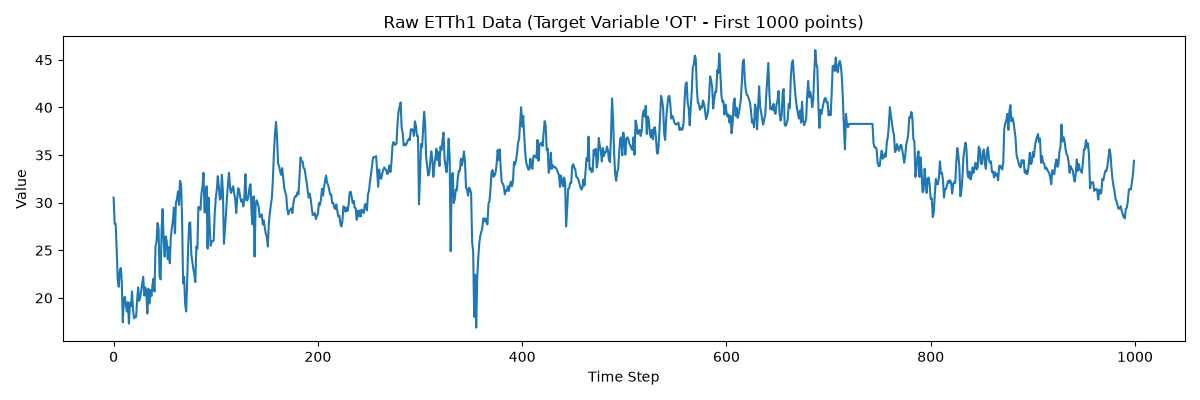
\includegraphics[width=\linewidth]{raw_data.png}
    \small (a) Raw ETTh1 OT series sample.
\end{minipage}\hfill
\begin{minipage}{0.47\textwidth}
    \centering
    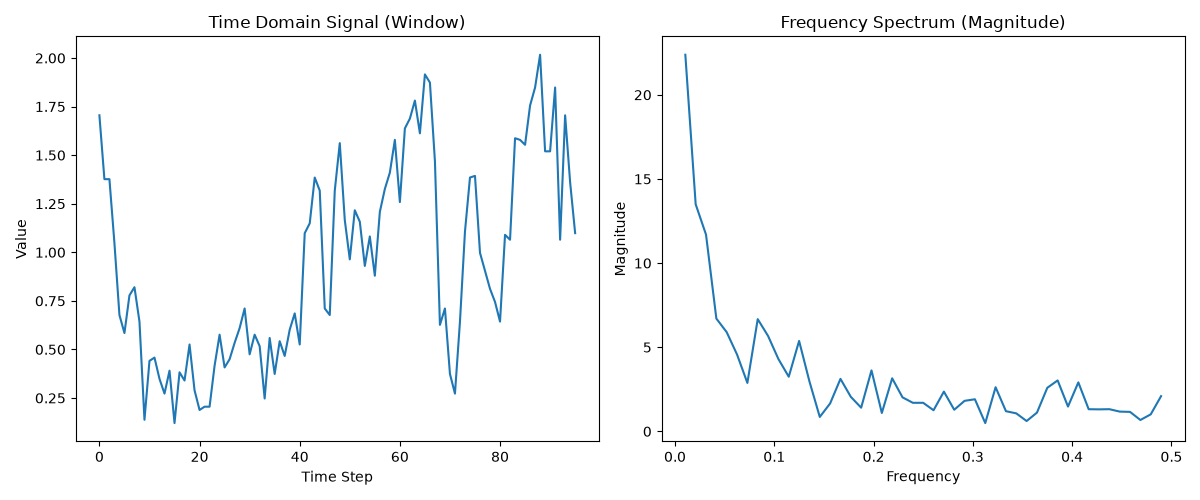
\includegraphics[width=\linewidth]{frequency_analysis.png}
    \small (b) Time window and FFT magnitude spectrum.
\end{minipage}
\caption{Data and frequency visualizations generated by the project.}
\label{fig:rawfreq}
\end{figure*}

\section{FAN Method}
\subsection{Frequency Decomposition}
For each batch, channel, and input window, the implementation applies a real-valued fast Fourier transform along the time dimension. For one channel, the discrete transform is
\begin{equation}
X_k=\sum_{t=0}^{L-1}x_t e^{-j2\pi kt/L}.
\end{equation}
The magnitudes $|X_k|$ are ranked and a binary mask retains the $K$ largest components. If $\mathcal{K}$ denotes their indices, the filtered spectrum is
\begin{equation}
\widetilde{X}_k=
\begin{cases}
X_k, & k\in\mathcal{K},\\
0, & \text{otherwise}.
\end{cases}
\end{equation}
An inverse real FFT reconstructs the dominant component
$\mathbf{X}_{\mathrm{freq}}$, and the residual is
\begin{equation}
\mathbf{X}_{\mathrm{res}}=
\mathbf{X}-\mathbf{X}_{\mathrm{freq}}.
\label{eq:residual}
\end{equation}
The main experiments use $K=5$. Figure~\ref{fig:reconstruction} illustrates Top-K reconstruction on a training window.

\begin{figure}[t]
\centering
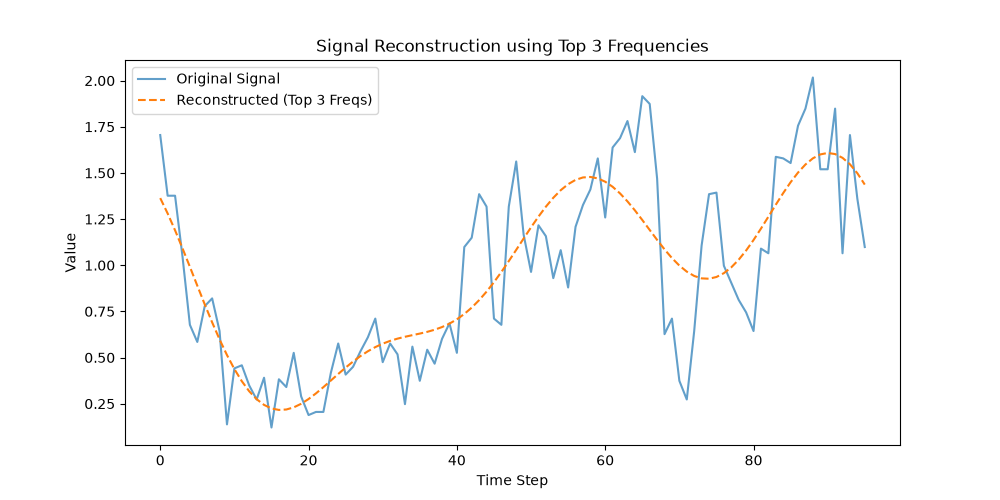
\includegraphics[width=0.96\columnwidth]{reconstruction_demo.png}
\caption{Repository demonstration of frequency-based signal reconstruction.}
\label{fig:reconstruction}
\end{figure}

\subsection{Residual Forecasting Backbone}
The integrated FAN model uses a simple linear backbone. The tensor is transposed so that one shared linear mapping operates on the time dimension of every feature:
\begin{equation}
\widehat{\mathbf{Y}}_{\mathrm{res}}
=B(\mathbf{X}_{\mathrm{res}}),
\qquad B:\mathbb{R}^{96}\rightarrow\mathbb{R}^{H}.
\end{equation}
This predicts the future residual component.

\subsection{Dominant-Component Prediction}
The removed component is predicted separately. For every channel, the MLP maps the length-96 dominant component to 64 hidden values, concatenates these values with the original length-96 input, maps the resulting 160 values to 128 hidden units, and finally produces $H$ future values. ReLU activation is used after the first two linear layers. This produces
$\widehat{\mathbf{Y}}_{\mathrm{freq}}$.

\subsection{Adaptive Denormalization}
The final forecast recombines both paths:
\begin{equation}
\widehat{\mathbf{Y}}=
\widehat{\mathbf{Y}}_{\mathrm{res}}+
\widehat{\mathbf{Y}}_{\mathrm{freq}}.
\label{eq:combine}
\end{equation}
Thus the backbone does not need to model the extracted dominant component by itself.

\begin{figure}[t]
\centering
\resizebox{0.96\columnwidth}{!}{%
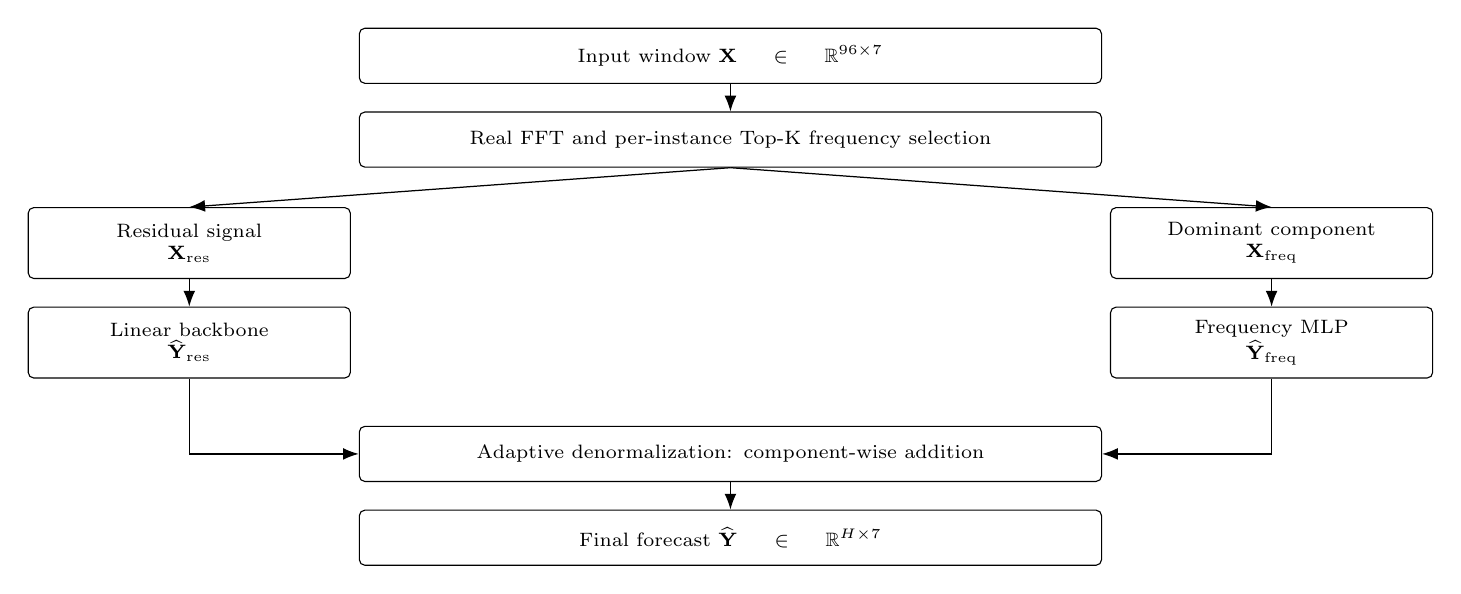
\begin{tikzpicture}[
    node distance=3.5mm and 4mm,
    flow/.style={-{Latex[length=2mm]}, line width=0.45pt},
    stage/.style={draw, rounded corners=2pt, align=center,
        minimum height=7mm, text width=0.76\columnwidth,
        inner sep=3pt, font=\scriptsize},
    branch/.style={draw, rounded corners=2pt, align=center,
        minimum height=9mm, text width=0.32\columnwidth,
        inner sep=3pt, font=\scriptsize}
]
\node[stage] (input) {Input window $\mathbf{X}\in\mathbb{R}^{96\times7}$};
\node[stage, below=of input] (fft) {Real FFT and per-instance Top-K frequency selection};

\node[branch, below left=5mm and 1mm of fft] (residual)
    {Residual signal\\$\mathbf{X}_{\mathrm{res}}$};
\node[branch, below right=5mm and 1mm of fft] (dominant)
    {Dominant component\\$\mathbf{X}_{\mathrm{freq}}$};

\node[branch, below=of residual] (backbone)
    {Linear backbone\\$\widehat{\mathbf{Y}}_{\mathrm{res}}$};
\node[branch, below=of dominant] (mlp)
    {Frequency MLP\\$\widehat{\mathbf{Y}}_{\mathrm{freq}}$};

\coordinate (branchmid) at ($(backbone.south)!0.5!(mlp.south)$);
\node[stage, below=6mm of branchmid] (combine)
    {Adaptive denormalization: component-wise addition};
\node[stage, below=of combine] (output)
    {Final forecast $\widehat{\mathbf{Y}}\in\mathbb{R}^{H\times7}$};

\draw[flow] (input) -- (fft);
\draw[flow] (fft.south) -- (residual.north);
\draw[flow] (fft.south) -- (dominant.north);
\draw[flow] (residual) -- (backbone);
\draw[flow] (dominant) -- (mlp);
\draw[flow] (backbone.south) |- (combine.west);
\draw[flow] (mlp.south) |- (combine.east);
\draw[flow] (combine) -- (output);
\end{tikzpicture}
}
\caption{Control flow of the implemented FAN-integrated forecasting model.}
\label{fig:pipeline}
\end{figure}

\section{Baseline Model}
The project implements DLinear as its comparison baseline. A moving average with kernel size 25 decomposes the input into seasonal and trend components. Independent linear time projections forecast both parts, and their outputs are added. The same dataset split, sequence length, horizon, optimizer, loss, and evaluation code are used for DLinear and FAN, providing a controlled project-level comparison.

\section{Training and Evaluation}
Table~\ref{tab:settings} lists the recorded experimental settings. The Adam optimizer minimizes mean squared error. At the end of training, the state with the lowest validation MSE among the three epochs is restored. Test evaluation processes every batch and weights errors by the number of tensor elements, including the shorter final batch.

\begin{table}[t]
\caption{Experimental configuration}
\label{tab:settings}
\centering
\footnotesize
\begin{tabular}{@{}p{0.52\columnwidth}p{0.39\columnwidth}@{}}
\toprule
Setting & Value\\
\midrule
Input length & 96\\
Prediction horizons & 12 to 96, step 12\\
Input/output channels & 7 / 7\\
Training epochs & 3\\
Batch size & 32\\
Optimizer & Adam\\
Learning rate & 0.001\\
Training objective & MSE\\
Main FAN Top-K & 5\\
Random seed & 42\\
Execution device & CPU\\
Evaluation coverage & Complete test loaders\\
\bottomrule
\end{tabular}
\end{table}

For $N$ forecast elements, the reported metrics are
\begin{equation}
\mathrm{MSE}=\frac{1}{N}\sum_{i=1}^{N}(y_i-\hat{y}_i)^2,
\qquad
\mathrm{MAE}=\frac{1}{N}\sum_{i=1}^{N}|y_i-\hat{y}_i|.
\end{equation}
The evaluation covers four datasets, two models, and eight horizons, producing 64 main configurations. Checkpoints and both CSV and JSON result files are persisted for reproducibility.

\section{Results and Discussion}
\subsection{Dataset Comparison at Horizon 24}
Table~\ref{tab:mainresults} reports full test-set results at horizon 24. FAN records the lower MSE on ETTh1 and ETTm2, while DLinear records the lower MSE on ETTh2 and ETTm1. FAN's lowest MSE in this table is 0.0577 on ETTm2. The result does not support a claim that either model wins on every dataset.

\begin{table}[t]
\caption{Full test-set results at prediction horizon 24}
\label{tab:mainresults}
\centering
\footnotesize
\begin{tabular}{@{}llrr@{}}
\toprule
Dataset & Model & MSE & MAE\\
\midrule
ETTh1 & FAN & \textbf{0.2995} & 0.3739\\
      & DLinear & 0.3058 & \textbf{0.3716}\\
ETTh2 & FAN & 0.0831 & 0.2061\\
      & DLinear & \textbf{0.0816} & \textbf{0.2026}\\
ETTm1 & FAN & 0.2736 & 0.3403\\
      & DLinear & \textbf{0.2507} & \textbf{0.3314}\\
ETTm2 & FAN & \textbf{0.0577} & \textbf{0.1687}\\
      & DLinear & 0.0600 & 0.1713\\
\bottomrule
\end{tabular}
\end{table}

\subsection{Forecast-Horizon Comparison}
Figure~\ref{fig:modelcomparison} summarizes MSE over all eight horizons. ETTh1 shows FAN below DLinear for every tested MSE point. On ETTh2 the curves are close and alternate. DLinear is lower on most ETTm1 horizons, whereas FAN is lower on most ETTm2 horizons. Error generally increases as the forecast horizon becomes longer, although not every dataset is strictly monotonic at every point.

\begin{figure*}[t]
\centering
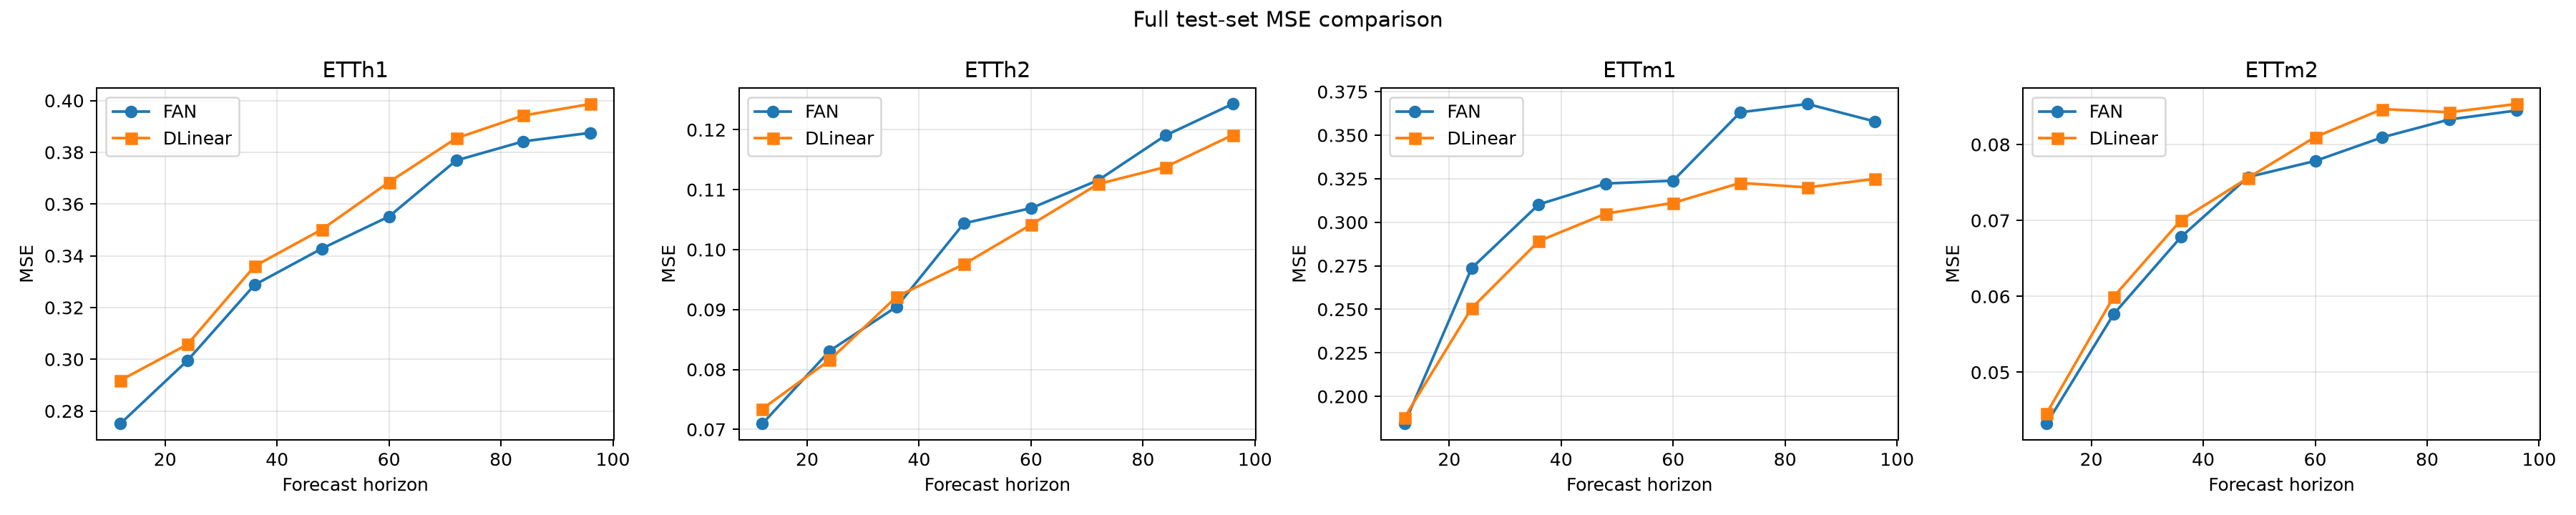
\includegraphics[width=0.96\textwidth]{model_comparison_mse.png}
\caption{Full test-set MSE for FAN and DLinear across four datasets and eight horizons.}
\label{fig:modelcomparison}
\end{figure*}

Table~\ref{tab:etth1horizons} gives the corresponding ETTh1 values. FAN's MSE advantage remains modest, and the MAE values of the two models are close at several horizons.

\begin{table}[t]
\caption{ETTh1 results across forecast horizons}
\label{tab:etth1horizons}
\centering
\scriptsize
\setlength{\tabcolsep}{3.5pt}
\begin{tabular}{@{}rrrrr@{}}
\toprule
$H$ & FAN MSE & FAN MAE & DL MSE & DL MAE\\
\midrule
12 & 0.2751 & 0.3578 & 0.2918 & 0.3656\\
24 & 0.2995 & 0.3739 & 0.3058 & 0.3716\\
36 & 0.3288 & 0.3924 & 0.3360 & 0.3936\\
48 & 0.3428 & 0.4019 & 0.3502 & 0.4016\\
60 & 0.3552 & 0.4105 & 0.3684 & 0.4149\\
72 & 0.3768 & 0.4269 & 0.3854 & 0.4266\\
84 & 0.3842 & 0.4325 & 0.3942 & 0.4326\\
96 & 0.3875 & 0.4354 & 0.3987 & 0.4353\\
\bottomrule
\end{tabular}
\end{table}

\subsection{Top-K Ablation}
The repository trains separate ETTh1 FAN models with
$K\in\{1,3,5,10,20\}$ at horizon 24. Table~\ref{tab:ablation} and Fig.~\ref{fig:ablation} show a small improvement over the tested range. $K=20$ records the lowest MSE and MAE. The differences are modest and concern one dataset and one seeded run; they do not establish a universal optimum.

\begin{table}[t]
\caption{ETTh1 Top-K ablation at horizon 24}
\label{tab:ablation}
\centering
\footnotesize
\begin{tabular}{@{}rrr@{}}
\toprule
Top-K & MSE & MAE\\
\midrule
1  & 0.3002 & 0.3736\\
3  & 0.2972 & 0.3738\\
5  & 0.2981 & 0.3739\\
10 & 0.2958 & 0.3720\\
20 & \textbf{0.2948} & \textbf{0.3718}\\
\bottomrule
\end{tabular}
\end{table}

\begin{figure}[t]
\centering
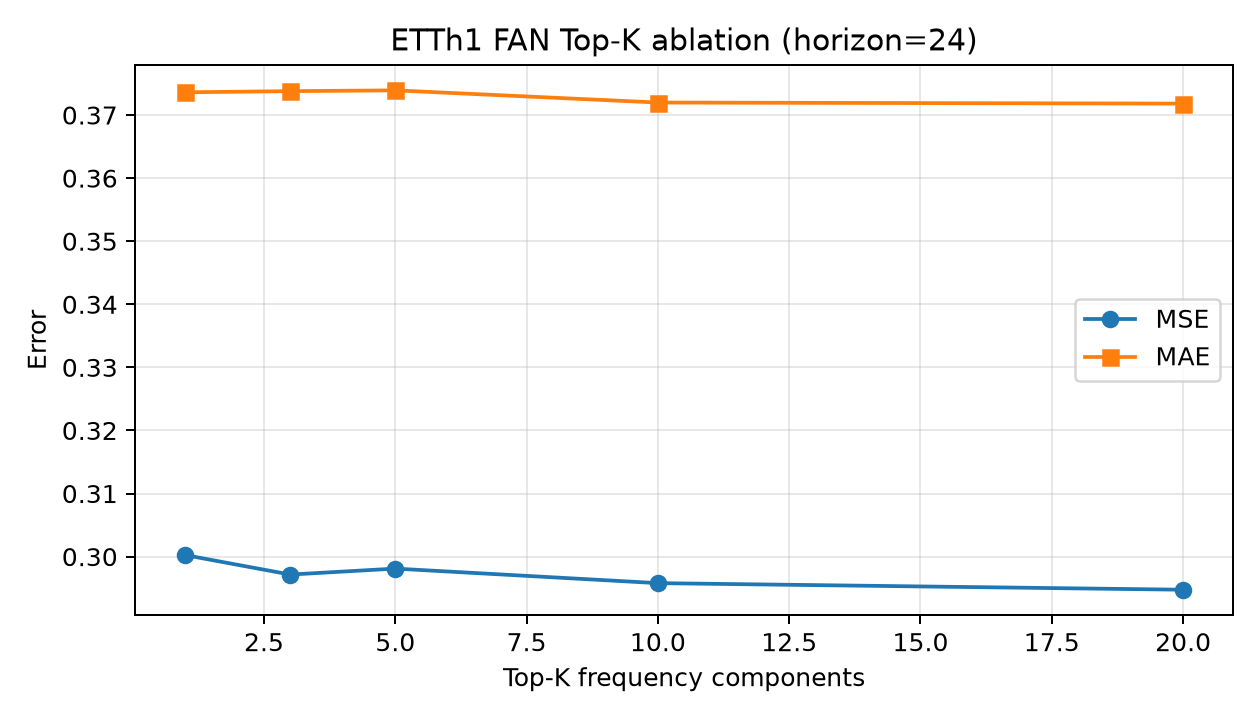
\includegraphics[width=0.96\columnwidth]{ablation_topk.png}
\caption{Recorded MSE and MAE for the ETTh1 Top-K ablation.}
\label{fig:ablation}
\end{figure}

\subsection{Forecast Visualization}
Figure~\ref{fig:forecast} presents one normalized OT example from the first ETTh1 test window. Both models follow part of the future movement, but their trajectories differ from the ground truth. This example supports qualitative inspection only; the aggregate metrics in Table~\ref{tab:mainresults} cover all test windows and channels.

\begin{figure}[t]
\centering
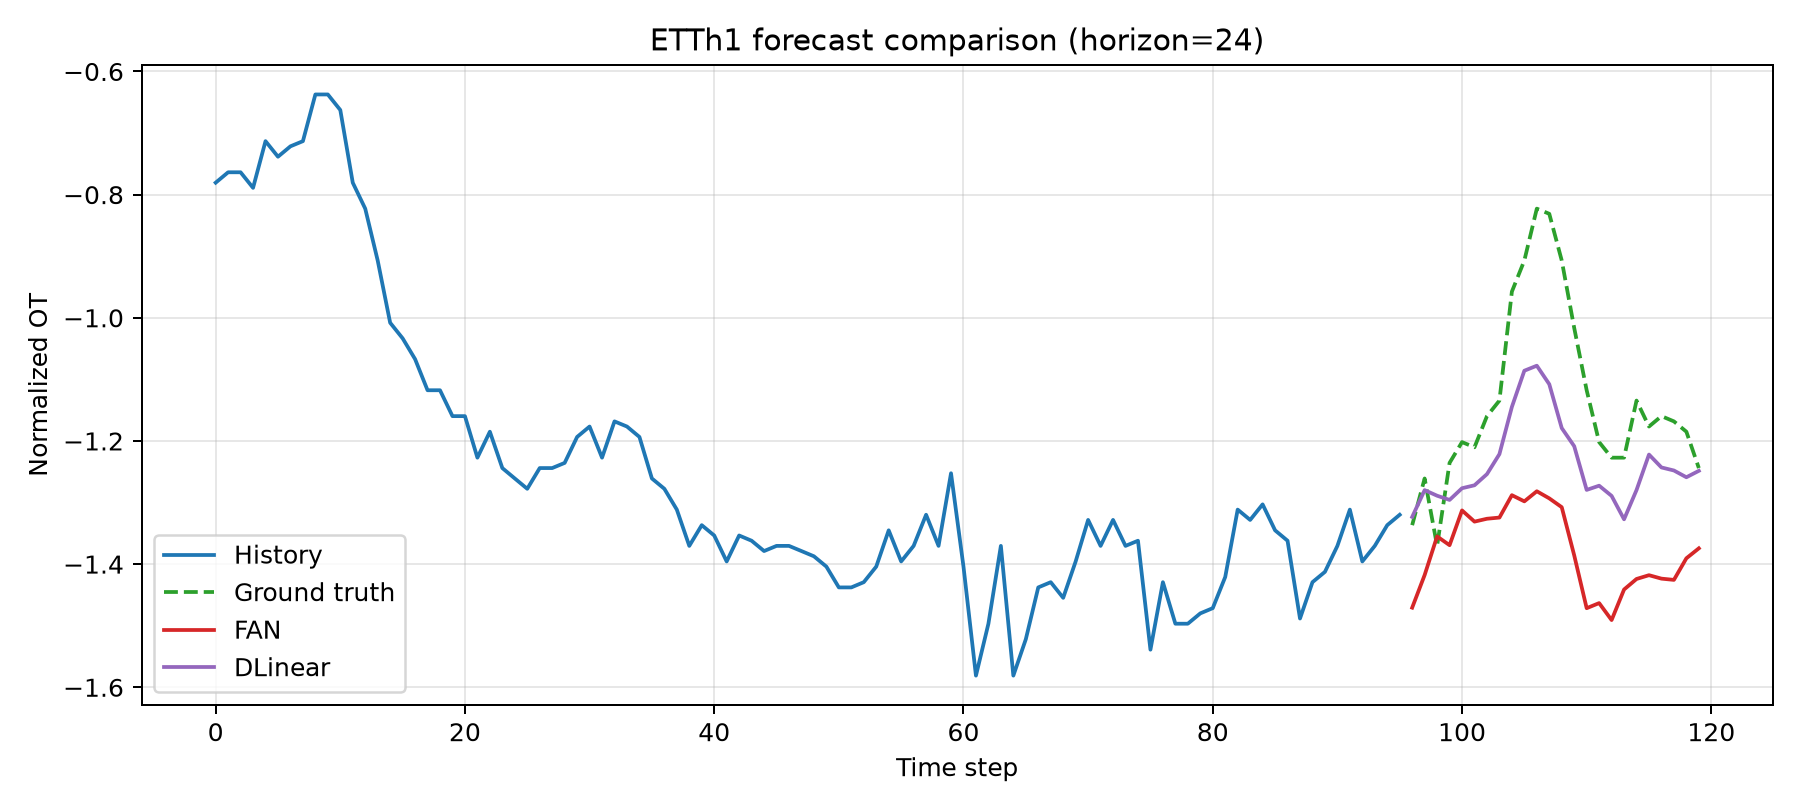
\includegraphics[width=0.96\columnwidth]{forecast_ETTh1_24.png}
\caption{ETTh1 OT forecast example at horizon 24 using reloaded checkpoints.}
\label{fig:forecast}
\end{figure}

\section{Interactive Application}
The project includes a minimalist Gradio interface implemented in \texttt{app.py}. The front end provides a dataset selector, a model selector, a horizon slider, an optional CSV upload, a Run Forecast button, a Matplotlib plot, and a metrics panel. No decorative images or icon-heavy controls are required.

The backend loads an \texttt{ETTDataset}, applies the same chronological splitting and training-only scaling used by the experiments, creates the selected FAN or DLinear model, and reloads the checkpoint matching the chosen dataset and horizon. The application then forecasts the first test window and plots normalized OT history, ground truth, and prediction. The displayed MSE and MAE are OT-only metrics for that one example, so they should not be confused with the full multivariate test metrics.

If no file is uploaded, the interface uses the selected bundled dataset. An uploaded file must use the ETT schema and exact feature order
\texttt{HUFL, HULL, MUFL, MULL, LUFL, LULL, OT}, with an optional \texttt{date} column. It must also contain enough rows for the selected sequence and horizon. The uploaded CSV supplies the data, while the dataset dropdown selects which pretrained checkpoint is used. Consequently, an uploaded file should follow the distribution of the selected checkpoint's dataset. Invalid, missing, non-numeric, non-finite, incorrectly ordered, or insufficient data produce an interface error instead of a silent forecast.

\section{Verification and Reproducibility}
Six automated tests verify frequency decomposition and reconstruction, odd-length FFT handling, FAN and DLinear output shapes, invalid mode and Top-K rejection, training-only scaler statistics, complete training/evaluation execution, and successful reload of all 64 UI checkpoints. The Gradio server was also launched locally and returned HTTP status 200.

The main reproduction commands are:
\begin{verbatim}
python scripts/train_all.py
python scripts/evaluate_all.py
python scripts/run_ablation.py
python -m unittest discover -s tests -v
python app.py
\end{verbatim}
The training script writes checkpoints to \texttt{outputs/models/}; the evaluation and ablation scripts write CSV and JSON records to \texttt{outputs/results/} and figures to \texttt{outputs/figures/}.

\section{Limitations and Future Work}
The experiments intentionally use three CPU epochs. Although the best validation state is retained, this training budget does not demonstrate full convergence. Each configuration has one seeded run, so the project does not estimate run-to-run variance or confidence intervals.

The FAN-integrated model uses the repository's simple linear backbone, and the only comparison baseline is DLinear. Additional backbone models are outside the completed scope. The aggregate metrics are calculated in standardized space across all seven channels rather than in original physical units. The Top-K ablation covers only ETTh1 at horizon 24.

The upload workflow reuses a selected pretrained checkpoint; it does not retrain on arbitrary uploaded data. Distributionally different CSV files can therefore give unreliable predictions even if their column shape is valid. Future work could add explicit dataset identification, inverse-scaled metrics, repeated trials, longer training, more backbones, and broader datasets. These extensions should retain the same leakage-safe scaling and full-test evaluation protocol.

\section{Conclusion}
This project implements an end-to-end FAN forecasting system rather than only a frequency-analysis demonstration. The completed pipeline performs leakage-safe preprocessing, instance-wise FFT decomposition, Top-K component extraction, residual forecasting, dominant-component prediction, adaptive recombination, baseline comparison, checkpoint persistence, full-loader evaluation, ablation analysis, automated testing, and interactive inference. The measured results show that FAN is competitive with DLinear but that the better model depends on the dataset and metric. This bounded conclusion is supported directly by the saved repository outputs and avoids transferring unverified performance claims from the original paper.

\balance
\begin{thebibliography}{3}
\bibitem{fanpaper}
W. Ye, S. Deng, Q. Zou, and N. Gui,
``Frequency Adaptive Normalization for Non-stationary Time Series Forecasting,''
in \emph{Advances in Neural Information Processing Systems}, 2024. [Online]. Available:
\url{https://proceedings.neurips.cc/paper_files/paper/2024/file/37c6d0bc4d2917dcbea693b18504bd87-Paper-Conference.pdf}

\bibitem{ettdataset}
ETDataset contributors, ``ETDataset: Electricity Transformer Temperature data,'' GitHub repository. [Online]. Available:
\url{https://github.com/zhouhaoyi/ETDataset}

\bibitem{fancode}
FAN project team, ``Frequency Adaptive Normalization for Non-Stationary Time-Series Forecasting,'' GitHub repository. [Online]. Available:
\url{https://github.com/meetdhorajiya/FAN}. Accessed: Sep. 24, 2026.

\end{thebibliography}

\end{document}
